% This file was created with tikzplotlib v0.10.1.
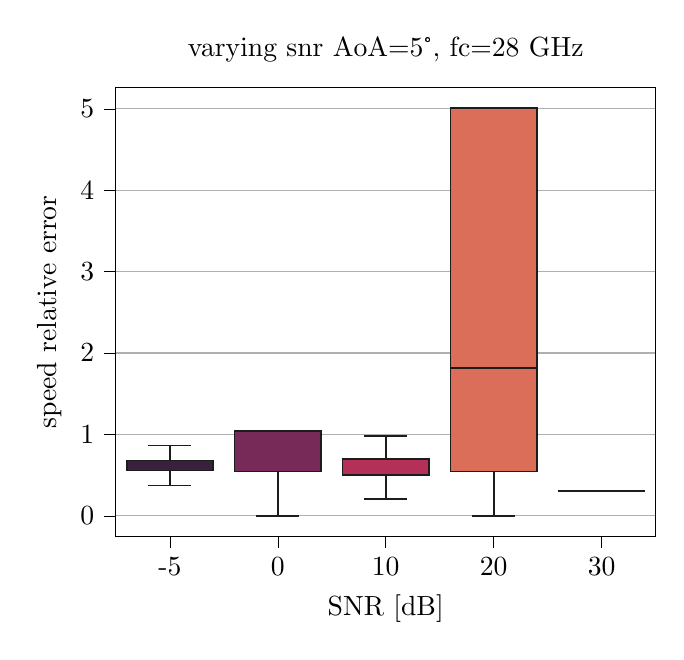
\begin{tikzpicture}

\definecolor{black28}{RGB}{28,28,28}
\definecolor{brown1814888}{RGB}{181,48,88}
\definecolor{burlywood231175145}{RGB}{231,175,145}
\definecolor{darkgray176}{RGB}{176,176,176}
\definecolor{darkslategray583162}{RGB}{58,31,62}
\definecolor{indianred21811088}{RGB}{218,110,88}
\definecolor{purple1194288}{RGB}{119,42,88}

\begin{axis}[
tick align=outside,
tick pos=left,
title={varying snr AoA=5°, fc=28 GHz},
x grid style={darkgray176},
xlabel={SNR [dB]},
xmin=-0.5, xmax=4.5,
xtick style={color=black},
xtick={0,1,2,3,4},
xticklabels={-5,0,10,20,30},
y grid style={darkgray176},
ylabel={speed relative error},
ymajorgrids,
ymin=-0.250248890501401, ymax=5.25767203376294,
ytick style={color=black}
]
\path [draw=black28, fill=darkslategray583162, semithick]
(axis cs:-0.4,0.557459410403683)
--(axis cs:0.4,0.557459410403683)
--(axis cs:0.4,0.68057459144577)
--(axis cs:-0.4,0.68057459144577)
--(axis cs:-0.4,0.557459410403683)
--cycle;
\path [draw=black28, fill=purple1194288, semithick]
(axis cs:0.6,0.543050375943074)
--(axis cs:1.4,0.543050375943074)
--(axis cs:1.4,1.04229995321923)
--(axis cs:0.6,1.04229995321923)
--(axis cs:0.6,0.543050375943074)
--cycle;
\path [draw=black28, fill=brown1814888, semithick]
(axis cs:1.6,0.501656053590428)
--(axis cs:2.4,0.501656053590428)
--(axis cs:2.4,0.697864101259948)
--(axis cs:1.6,0.697864101259948)
--(axis cs:1.6,0.501656053590428)
--cycle;
\path [draw=black28, fill=indianred21811088, semithick]
(axis cs:2.6,0.543828775010864)
--(axis cs:3.4,0.543828775010864)
--(axis cs:3.4,5.00731169757774)
--(axis cs:2.6,5.00731169757774)
--(axis cs:2.6,0.543828775010864)
--cycle;
\path [draw=black28, fill=burlywood231175145, semithick]
(axis cs:3.6,0.302788689908093)
--(axis cs:4.4,0.302788689908093)
--(axis cs:4.4,0.302788692186846)
--(axis cs:3.6,0.302788692186846)
--(axis cs:3.6,0.302788689908093)
--cycle;
\addplot [semithick, black28]
table {%
0 0.557459410403683
0 0.372875989161795
};
\addplot [semithick, black28]
table {%
0 0.68057459144577
0 0.865097335428962
};
\addplot [semithick, black28]
table {%
-0.2 0.372875989161795
0.2 0.372875989161795
};
\addplot [semithick, black28]
table {%
-0.2 0.865097335428962
0.2 0.865097335428962
};
\addplot [semithick, black28]
table {%
1 0.543050375943074
1 0.000111151510614517
};
\addplot [semithick, black28]
table {%
1 1.04229995321923
1 1.04229995321926
};
\addplot [semithick, black28]
table {%
0.8 0.000111151510614517
1.2 0.000111151510614517
};
\addplot [semithick, black28]
table {%
0.8 1.04229995321926
1.2 1.04229995321926
};
\addplot [semithick, black28]
table {%
2 0.501656053590428
2 0.20758022774296
};
\addplot [semithick, black28]
table {%
2 0.697864101259948
2 0.979775952518031
};
\addplot [semithick, black28]
table {%
1.8 0.20758022774296
2.2 0.20758022774296
};
\addplot [semithick, black28]
table {%
1.8 0.979775952518031
2.2 0.979775952518031
};
\addplot [semithick, black28]
table {%
3 0.543828775010864
3 0.00020029021789702
};
\addplot [semithick, black28]
table {%
3 5.00731169757774
3 5.00731199175093
};
\addplot [semithick, black28]
table {%
2.8 0.00020029021789702
3.2 0.00020029021789702
};
\addplot [semithick, black28]
table {%
2.8 5.00731199175093
3.2 5.00731199175093
};
\addplot [semithick, black28]
table {%
4 0.302788689908093
4 0.302788686504341
};
\addplot [semithick, black28]
table {%
4 0.302788692186846
4 0.302788692186846
};
\addplot [semithick, black28]
table {%
3.8 0.302788686504341
4.2 0.302788686504341
};
\addplot [semithick, black28]
table {%
3.8 0.302788692186846
4.2 0.302788692186846
};
\addplot [semithick, black28]
table {%
-0.4 0.680574591380663
0.4 0.680574591380663
};
\addplot [semithick, black28]
table {%
0.6 1.04229994421236
1.4 1.04229994421236
};
\addplot [semithick, black28]
table {%
1.6 0.697864101144677
2.4 0.697864101144677
};
\addplot [semithick, black28]
table {%
2.6 1.8123902820333
3.4 1.8123902820333
};
\addplot [semithick, black28]
table {%
3.6 0.302788692186809
4.4 0.302788692186809
};
\end{axis}

\end{tikzpicture}
